\section{設計}

本章では、従来のクラウドゲーミングにおいてクラウドのデータセンターとプレイヤー端末間の遅延を避けることができないという課題を解決するための、ボランティアコンピューティング資源を活用するクラウドゲーミングシステムを提案する。
まず提案システムの概要を述べた後、システムを実装するに当たっての課題について述べる。最後にシステムを構成するコンポーネントとその役割について述べる。

\subsection{提案システムの概要}
提案システムの概要を図\ref{fig:arch}に示す。提案システムは、クラウドのデータセンターに比べてより近いボランティアが提供する遊休コンピュータでクラウドゲームサーバをホストする。それにより、プレイヤーがクラウドゲーミングのプレイを通して体験する遅延を削減ということを目的とするものである。

システムの構成要素として、プレイヤーPC、クラウド上のボランティアクラウドゲーミングコントローラ、およびボランティアが提供する遊休コンピュータの3つのハードウェアがある。プレイヤーPCは、クラウドゲーミングをプレイするプレイヤーの所有するPCである。遊休コンピュータはボランティアが所有しているコンピュータの、一時的に使用していないコンピュータリソースを貸与している状態のものを指す。ボランティアクラウドゲーミングコントローラはプレイヤーPCと遊休コンピュータのマッチングを行う。

それぞれのハードウェアで動作するソフトウェアの構成要素について述べる。プレイヤーPCで動作するボランティアクラウド(VC)クライアントエージェントは、プレイヤーの希望に応じてボランティアクラウドゲーミングコントローラにゲームプレイを要求する。ボランティアクラウドゲーミングコントローラ上で動作するVCコントローラは、プレイヤーPCから要求を受け取ると遊休コンピュータとのマッチングを行う。遊休コンピュータ上で動作するVCホストエージェントは、VCコントローラからのクラウドゲームの実行要求に応じてクラウドゲームサーバの起動を行う。クラウドゲームサーバとクラウドゲームクライアントは、遊休コンピュータとプレイヤーPCを直接接続してクラウドゲーミングのプレイを実現する。

%

%プレイヤーPC上のVCクライアントエージェントがクラウド上のVCコントローラにゲームプレイを要求。VCコントローラが遊休コンピュータにVCホストエージェントにクラウドゲームの実行を要求。遊休コンピュータでクラウドゲームサーバとゲームが起動し、プレイヤーPC上のクラウドゲームクライアントと通信してゲームをする。

\begin{figure*}[t]
    \centering
    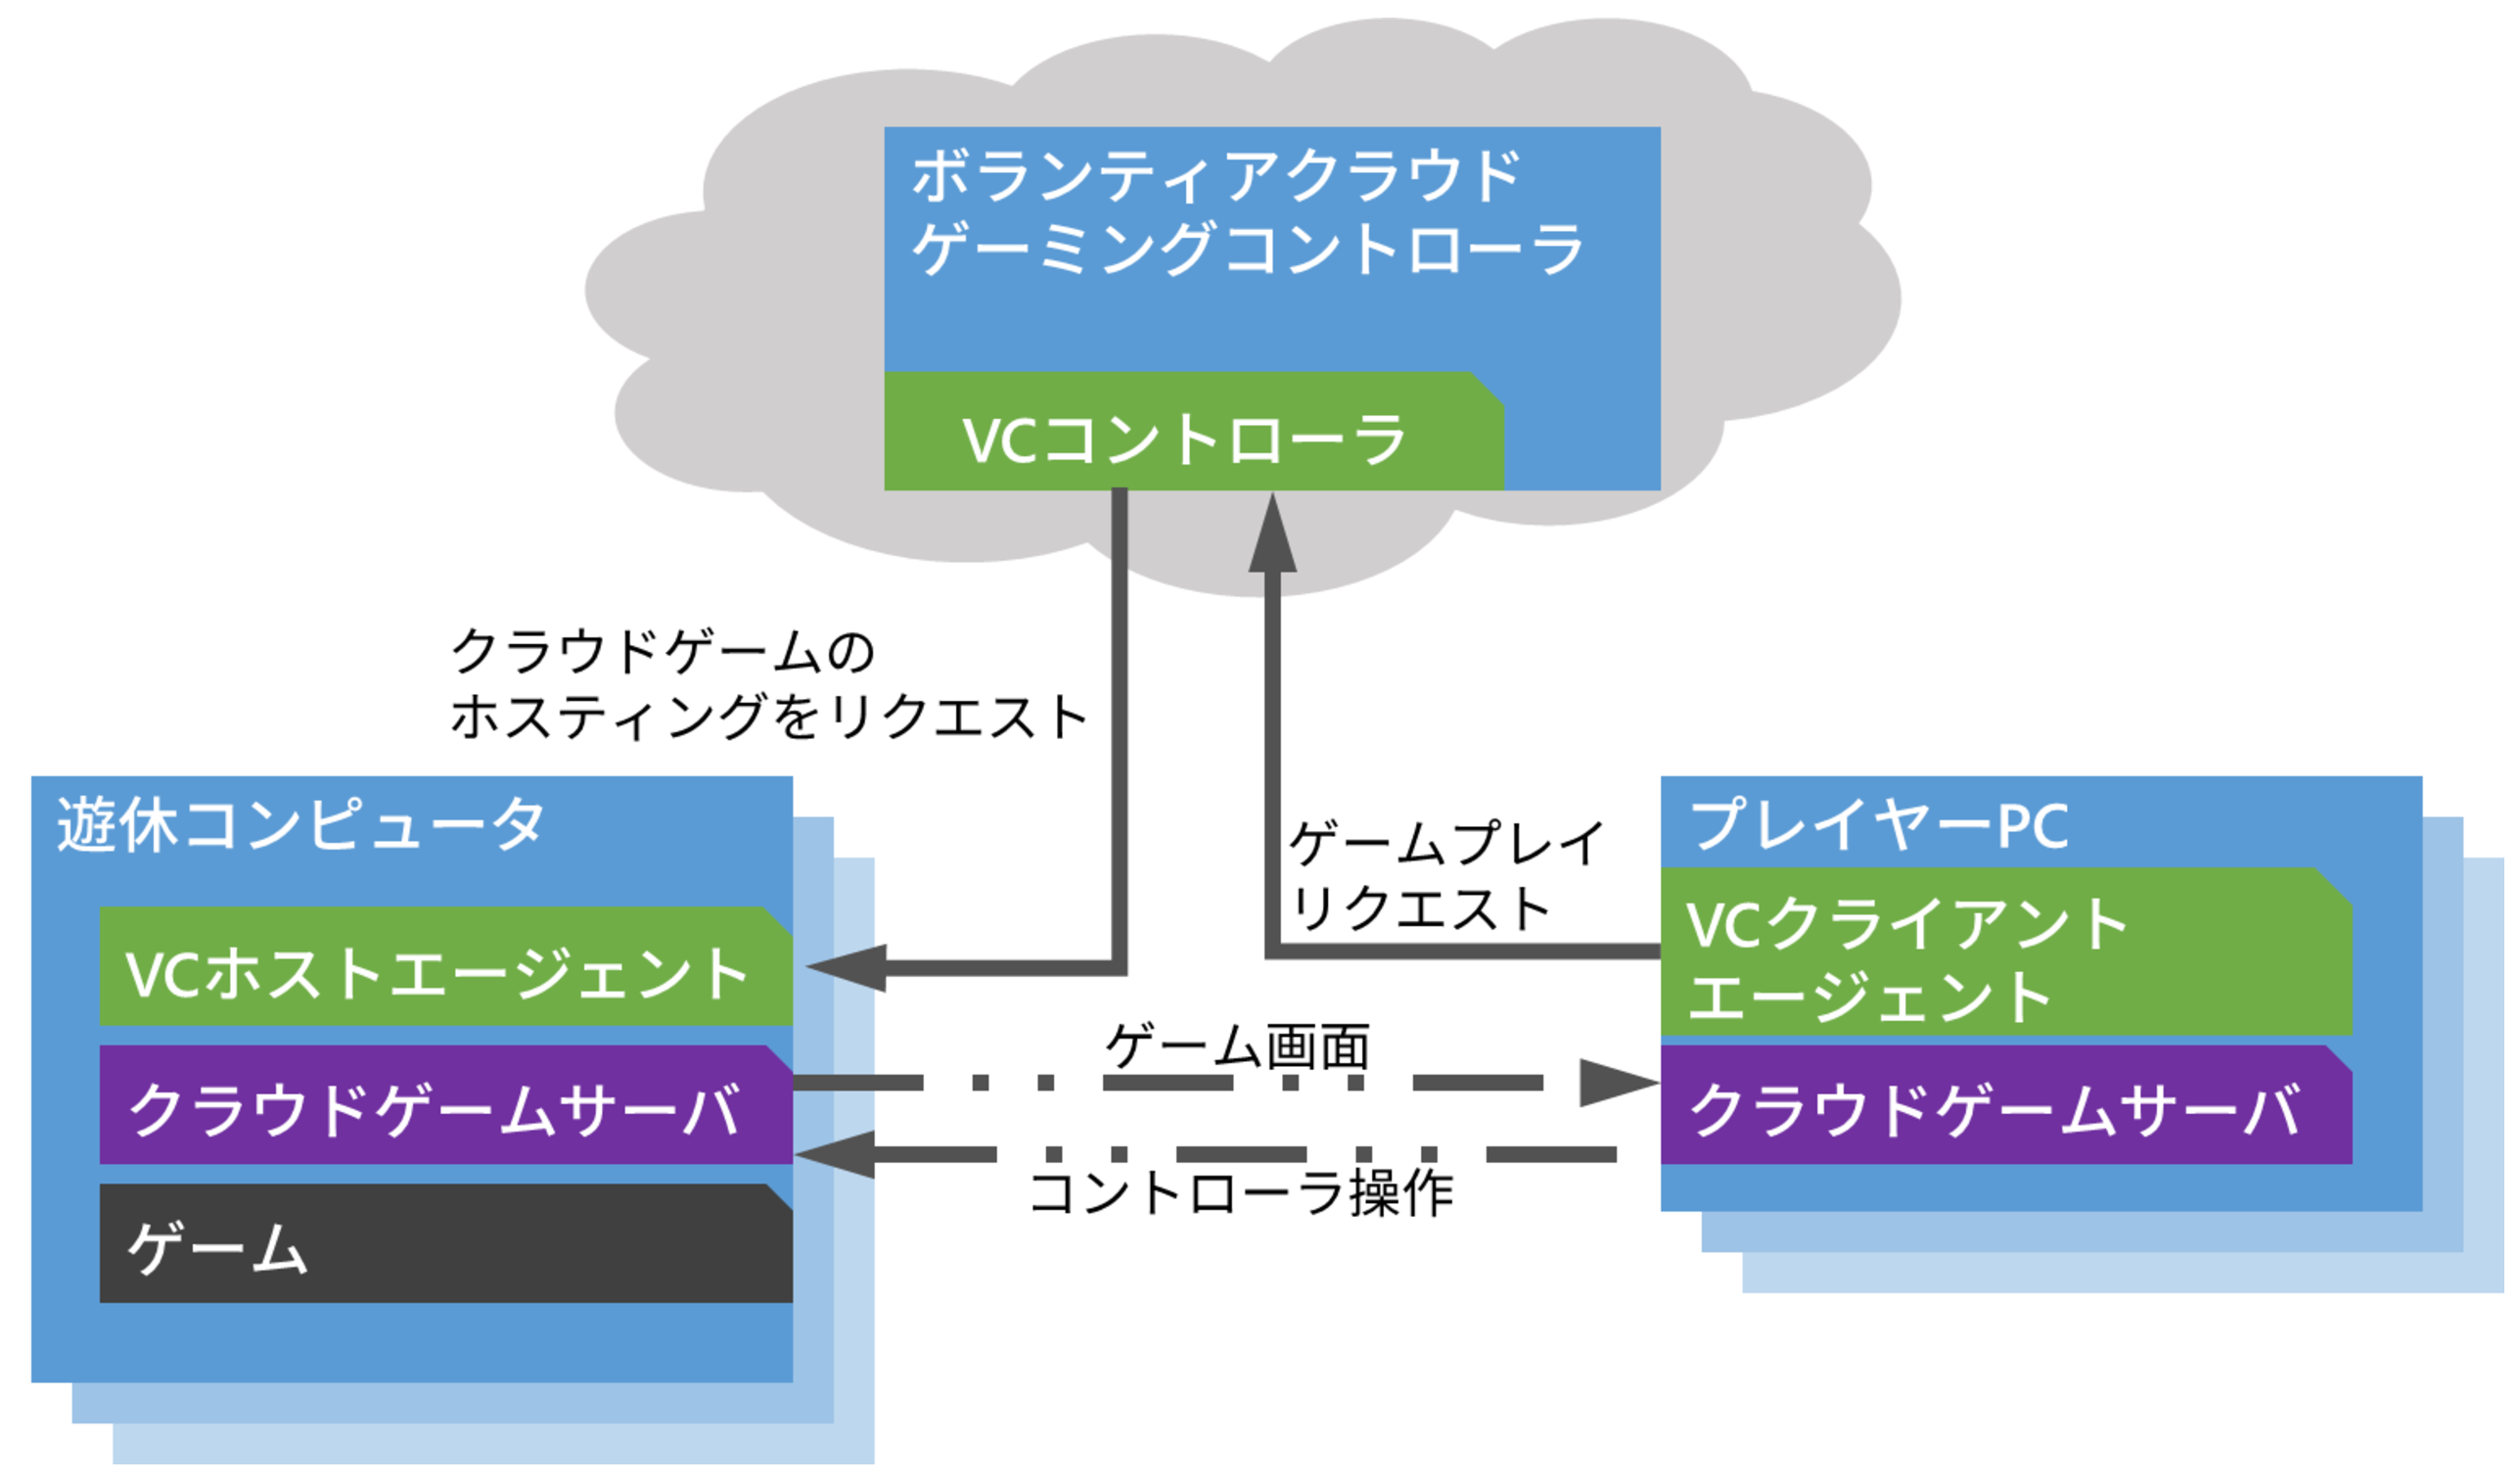
\includegraphics[width=0.8\textwidth,keepaspectratio,clip]{img/architecture.eps}
    \caption{提案システムの概要}
    \label{fig:arch}
\end{figure*}

\subsection{実装上の課題とアプローチ}
パブリッククラウドやビジネス向けのサーバでクラウドゲーミングサービスを提供する場合と異なり、提案システムはクラウドゲームサーバをボランティアの提供するユーザコンピュータ上で実行する。しかしユーザコンピュータはNATやファイアウォールの背後にあり、また固定IPアドレスを有しないことが一般的であるため遊休コンピュータとプレイヤーPCが直接通信することが困難である。そのため、提案システムの実装にあたり次の2点の課題が生じる。
\begin{itemize}
    \item クラウド上のコントローラから遊休コンピュータへクラウドゲームの実行等の直接命令を送ることができない
    \item クラウドゲームサーバ/クライアントを展開する遊休コンピュータとプレイヤーPC間での通信において、双方向的な直接通信を展開できない
\end{itemize}
コントローラと遊休コンピュータ間の通信については、RPCの技術を用いてトンネリングを行い、命令の伝送を行うことを試みる。クラウドゲームサーバ/クライアント間の通信については、P2P型のVPNを活用することでの接続を試みる。その性能についてネットワークとQoEの2つの観点から評価し、ボランティアコンピューティングをクラウドゲーミングに利用することが有効な条件を本研究で明らかにする。

\subsection{構成コンポーネント}
本項では各構成要素の詳細を述べる。

\subsubsection{VCコントローラ}
クラウド上に配備するVCコントローラはゲームをプレイしたいプレイヤーのPCと利用可能な遊休コンピュータをマッチングする役割を果たす。主な機能は以下の通りである。
\begin{itemize}
    \item プレイヤーからのゲームプレイ要求を受け付ける
    \item 最適な遊休コンピュータを発見して割り当てる
    \item プレイヤーPCと遊休コンピュータが通信を確立するための接続情報を配布する
\end{itemize}
マッチングの要件として、プレイヤーPCと遊休コンピュータが接続する際のネットワーク遅延が小さいことがある。そのため、VCコントローラはプレイヤーからのゲームプレイ要求に基づき、利用可能な遊休コンピュータの中から最も遅延の小さくなるものを探す。

%プレイヤーPCからのゲームプレイの要求を受け取ると、利用可能な遊休コンピュータ群の中からプレイヤーPCからのネットワーク遅延が小さいものを見つける。そしてその遊休コンピュータに対してクラウドゲームの実行を要求する。また、このマッチングの成立後、VCコントローラはVCクライアントエージェントとVCホストエージェントにクラウドゲームサーバ/クライアントが通信するためのリンクを張るのに必要な情報を配布する。

\subsubsection{VCクライアントエージェント}
VCクライアントエージェントは、プレイヤーの希望に応じてボランティアクラウドゲーミングコントローラにゲームプレイの要求をする役割を持つ。プレイしたいゲームやサーバとリンクを張るために必要なネットワーク情報などを付帯して、VCコントローラへゲームプレイの要求を送信する。

\subsubsection{VCホストエージェント}
VCホストエージェントはVCコントローラの実行要求に応じてクラウドゲームサーバの起動を行う役割を果たす。また、プレイヤーが実際にプレイするゲームの起動も行う。起動が完了すると、接続に必要な情報と共にVCコントローラを経由してVCクライアントエージェントに起動完了の通知を送信する。

\subsubsection{クラウドゲームサーバ/クライアント}
クラウドゲームサーバ/クライアントは遊休コンピュータとプレイヤーPCを接続して、クラウドゲーミングのゲームプレイを提供する役割を果たす。クラウドゲームサーバはゲーム画面をキャプチャして、ビデオストリームとしてクラウドゲームクライアントに送信する。一方で、クラウドゲームクライアントは受け取ったゲーム画面の描画を行う。また、クラウドゲームクライアントはプレイヤーの入力操作をキャプチャしてクラウドゲームサーバ上のゲームの入力となるように送信を行う。

\subsection{提案システムの範囲及び制限}
提案システムには、ボランティアクラウドゲーミングコントローラにてプレイヤーPCと遊休コンピュータのマッチングを行う機能を含んでいる。しかし、プレイヤー端末とクラウドゲームサーバ間のネットワーク遅延に着目したマッチングは、既存のVM配置最適化\cite{placing}と同様の問題を扱うことになる。したがって本研究ではこの機能については対象外とし、ユーザコンピュータ間の通信によるクラウドゲーミングシステムの実現を主眼に置くこととする。